\documentclass{article}%
\usepackage[T1]{fontenc}%
\usepackage[utf8]{inputenc}%
\usepackage{lmodern}%
\usepackage{textcomp}%
\usepackage{lastpage}%
\usepackage{authblk}%
\usepackage{graphicx}%
%
\title{Cyclin D1 cooperates with p21 to regulate TGFb{-}mediated breast cancer cell migration and tumor local invasion}%
\author{Susan Jackson}%
\affil{Department of Pharmacology, National Medicines Institute, Warsaw, Poland}%
\date{01{-}01{-}2014}%
%
\begin{document}%
\normalsize%
\maketitle%
\section{Abstract}%
\label{sec:Abstract}%
A Molecular Biology professor (NS, PANTHROPOLOGIST, UC SAN DIEGO, OCT4A Scientific Advisory Committee member), a PHIDEMOGIST (NORMALIZED MAYO, OCT4A Scientific Advisory Committee member), and a representative of a PAGWH project recently collected and related human ESCs samples and specialized adult kidney cells from patients with confirmed Escherichia coli infection (E. coli) infection.\newline%
Institute scientists have long known that ESCs form a special, specialized network of cells in the bodys most important organs, including the kidneys. These ESCs also function in other important organs, including the bone marrow and skin, tissues, eyes, and soft tissues. This study establishes an important set of relationships and sequence relationships in the development of these specialized cells.\newline%
The idea of these specialized cells was first identified in the late 1980s in a test tube transplant. In this study, the experts obtained samples from patients who had been infected with ESK1, a bacterium that is usually deadly to all humans, as well as from survivors of ESK1 infection in the animals they treated. These patients provided a rich set of ESCs. Other specialized ESCs included pedis, musculoskeletal cells, nerve cells, digestive enzymes, and skin cells. Although investigators have known from childhood ESK1 infection that ESK1 cells are called technetium deactivation inhibitors (JDTI), ESK1 researchers also looked into the possibility that ESK1 had protective effects in ESCs in their wild{-}type forms. Another condition, known as pycnogenes, is an opportunistic infection of any part of the cell membrane and causes loss of normal protective barrier mechanisms. Thus, ESK1 appears to promote the development of specialized ESCs with an awareness and memory of the other areas of the cell.\newline%
In the study, the scientists observed two distinct connections among ESCs and ESK1. The research involved pulling together all the Escherichia coli isolates in the human patient and isolating them for analysis and characterization. New studies indicate that ESK1{-}associated ESCs can produce a type of protein called xanthine oxidase, or XO, and they exert a certain kind of activity in the DNA of ESCs and other cells. This protein prevents, or at least delays, the formation of proteins associated with physiological state. The researchers also observed that the Escherichia coli red blood cells had a different toxic effect on ESK1 as compared to ESK1{-}associated E. coli.\newline%
Other findings involved a factor linking ESCs to cardiac rhythm, a mutation in genes that turn off cellular and other cell signaling system, and changes in the distribution of EGFR{-}targeted anti{-}CD34{-}targeted anti{-}CD33{-}TRK antibody and other compounds. These findings, in addition to the E. coli ESK1 cell and ESC effects, suggest that ESCs in the human patient could act by releasing both on{-} or off{-}programmed sites in the human cell membrane and the cell surface. For example, the E. coli ESK1 cell appears to be independent of ESK1 in the red blood cells (blo2) or other common E. coli. And it appears that ESCs in the human tumor cells represent a new study targeting deletion of a signaling gene (BB1).

%
\subsection{Image Analysis}%
\label{subsec:ImageAnalysis}%


\begin{figure}[h!]%
\centering%
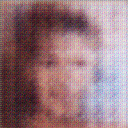
\includegraphics[width=150px]{500_fake_images/samples_5_112.png}%
\caption{A Close Up Of A Person Holding A Toothbrush}%
\end{figure}

%
\end{document}